%%%%%%%%%%%%%%%%%%%%%%%%%%%%%%%%%%%%%%%%%%%%%%%%%%%%%%%%%%%%%%%%%%
%%%%%%%% ICML 2015 EXAMPLE LATEX SUBMISSION FILE %%%%%%%%%%%%%%%%%
%%%%%%%%%%%%%%%%%%%%%%%%%%%%%%%%%%%%%%%%%%%%%%%%%%%%%%%%%%%%%%%%%%

% Use the following line _only_ if you're still using LaTeX 2.09.
%\documentstyle[icml2015,epsf,natbib]{article}
% If you rely on Latex2e packages, like most moden people use this:
\documentclass{article}

% use Times
\usepackage{times}
% For figures
\usepackage{graphicx} % more modern
%\usepackage{epsfig} % less modern
\usepackage{subfigure} 

% For citations
\usepackage{natbib}

% For algorithms
\usepackage{algorithm}
\usepackage{algorithmic}

% As of 2011, we use the hyperref package to produce hyperlinks in the
% resulting PDF.  If this breaks your system, please commend out the
% following usepackage line and replace \usepackage{icml2015} with
% \usepackage[nohyperref]{icml2015} above.
\usepackage{hyperref}

% Packages hyperref and algorithmic misbehave sometimes.  We can fix
% this with the following command.
\newcommand{\theHalgorithm}{\arabic{algorithm}}

% Employ the following version of the ``usepackage'' statement for
% submitting the draft version of the paper for review.  This will set
% the note in the first column to ``Under review.  Do not distribute.''
\usepackage{icml2015} 

% Employ this version of the ``usepackage'' statement after the paper has
% been accepted, when creating the final version.  This will set the
% note in the first column to ``Proceedings of the...''
%\usepackage[accepted]{icml2015}


% The \icmltitle you define below is probably too long as a header.
% Therefore, a short form for the running title is supplied here:
\icmltitlerunning{Submission and Formatting Instructions for ICML 2015}

\begin{document} 

\twocolumn[
\icmltitle{Title}

% It is OKAY to include author information, even for blind
% submissions: the style file will automatically remove it for you
% unless you've provided the [accepted] option to the icml2015
% package.
\icmlauthor{Noah Apthorpe, Josh Fass, Maithra Raghu}{}%{email@yourdomain.edu}
%\icmladdress{Your Fantastic Institute,
%           314159 Pi St., Palo Alto, CA 94306 USA}
%\icmlauthor{Your CoAuthor's Name}{email@coauthordomain.edu}
%\icmladdress{Their Fantastic Institute,
 %           27182 Exp St., Toronto, ON M6H 2T1 CANADA}

% You may provide any keywords that you 
% find helpful for describing your paper; these are used to populate 
% the "keywords" metadata in the PDF but will not be shown in the document
\icmlkeywords{boring formatting information, machine learning, ICML}

\vskip 0.3in
]

\begin{abstract} 
ABSTRACT ABSTRACT ABSTRACT
\end{abstract} 

\section{Introduction}
\label{sec:introduction}
Recent advances in computational biology have been driven by the development of experimental techniques that generate large datasets and corresponding machine learning algorithms for data analysis and interpretation.  

Mass cytometry is a particularly exciting modern technique that allows researchers to measure more than fifty molecular properties of millions of individual cells per experiment \cite{}.  Researchers can identify cell population heterogeneities ranging in scope from individual cells to complex hierarchical subpopulations. Such precision enables more detailed studies of many medically relevant phenomena, including identifying individual cells in specific disease states \cite{}, classifying cellular subpopulations by response to signalling perturbations \cite{}, understanding cellular reprogramming processes \cite{}, and investigating the natural heterogeneity of healthy systems \cite{}.  

However, the effectiveness of mass cytometry as an experimental tool depends on correctly interpreting the resulting high-dimensional datasets. To assist with data interpretation, researchers develop machine learning algorithms to calculate summary statistics or generate low-dimensional visualizations of raw data. In the case of mass cytometry, researchers are typically interested in three main analysis tasks, each corresponding to a machine learning task with biologically relevant constraints:

%\begin{table}[H]
%\begin{tabular}{p{0.2\linewidth}|p{0.2\linewidth}|p{0.2\linewidth}|p{0.2\linewidth}}
%\textbf{Analysis Goal} & \textbf{Machine Learning Task} & \textbf{Biological Constraints} & \textbf{Example Application}\\
\begin{enumerate}
\item Identifying and characterizing rare cellular subtypes -- Clustering --
Sensitivity to small clusters -- Identifying minimal residual disease 

\item Describe relations between cellular subtypes -- Structured output prediction -- Should not distort or artificially introduce structure into the results --  Monitoring clonal evolution in cancer 

\item Create human-readable representations to aid interpretation -- Low-dimensional embedding -- representations should be in 2D or 3D, either by means of a single structure-preserving projection or by decomposition into many low-dimensional projections -- Generating visual summaries for clinicians 
\end{enumerate}
%\end{tabular}
%\end{table}

Several domain-specific algorithms have been developed to address these analysis tasks, most notably SPADE \cite{}, FLOW-MAP \cite{}, Wanderlust \cite{}, DREMI/DREVI \cite{}, and viSNE \cite{}.  However, some limitations of these algorithms indicate the need for improved solutions.  First, none of these methods can be easily related to an underlying probabilistic model. This makes them prone to unpredictable structure-distorting behavior which can lead to misleading outputs. Second, these methods do not quantify how confident researchers should be when using the result to support experimental conclusions.

Here, we investigate SPADE, a widely used mass cytometry analysis algorithm,  and comment on its inconsistencies when applied to generated datasets with known ground truth (\S\ref{sec:spade}). This analysis indicates that SPADE may generate inaccurate results when applied to real datasets, suggesting the need for improvements.  We propose several improvements to the density-dependent downsampling component of SPADE  (\S\ref{sec:downsampling}), as well as an alternative approach to producing low-dimensional embeddings under similar constraints (\S\ref{sec:approximate_tpe}).   

 INCLUDE QUANTITATIVE IMPROVEMENTS ONCE SECTIONS ARE WRITTEN

\section{SPADE Inconsistency Analysis}
\label{sec:spade}
SPADE, or Spanning-tree Progression Analysis of Density-normalized Events \cite{} is a popular and influential algorithm for automating cell sub-population identification and visualization, directly from high-dimensional raw datasets. SPADE  (Figure~\ref{fig:spade_overview}) consists of the following multi-step data processing pipeline:

\begin{enumerate}
\item \textbf{Density Dependent Downsampling}: This simultaneously reduces computational load, and also ensures that rare cell sub-populations are not overshadowed by dominant larger cell clusters. 

\item \textbf{Clustering} The downsampled data is then used as input for agglomerative clustering, which groups individual cells in the dataset into sub-populations. 

\item \textbf{Cluster-preserving Up-sampling} Data omitted during downsampling is then assigned to identified sub-population clusters by a k-nearest-neighbors classifier.

\item \textbf{Minimum Spanning Tree Construction} To better understand relations between different subpopulations, a complete graph is constructed on the data with each cluster represented by its centroid and edge weights corresponding to Euclidean distance.  A minimum spanning tree is then computed on this underlying graph to pinpoint clusters which are especially ‘close’ to each other.
 
\item \textbf{Two Dimensional Embedding} To further aid visualization, the minimum spanning tree is then embedded in two dimensions using force-directed layout \cite{}. A plot of this embedding is then generated as the final output of SPADE.
\end{enumerate}

\begin{figure}
\begin{center}
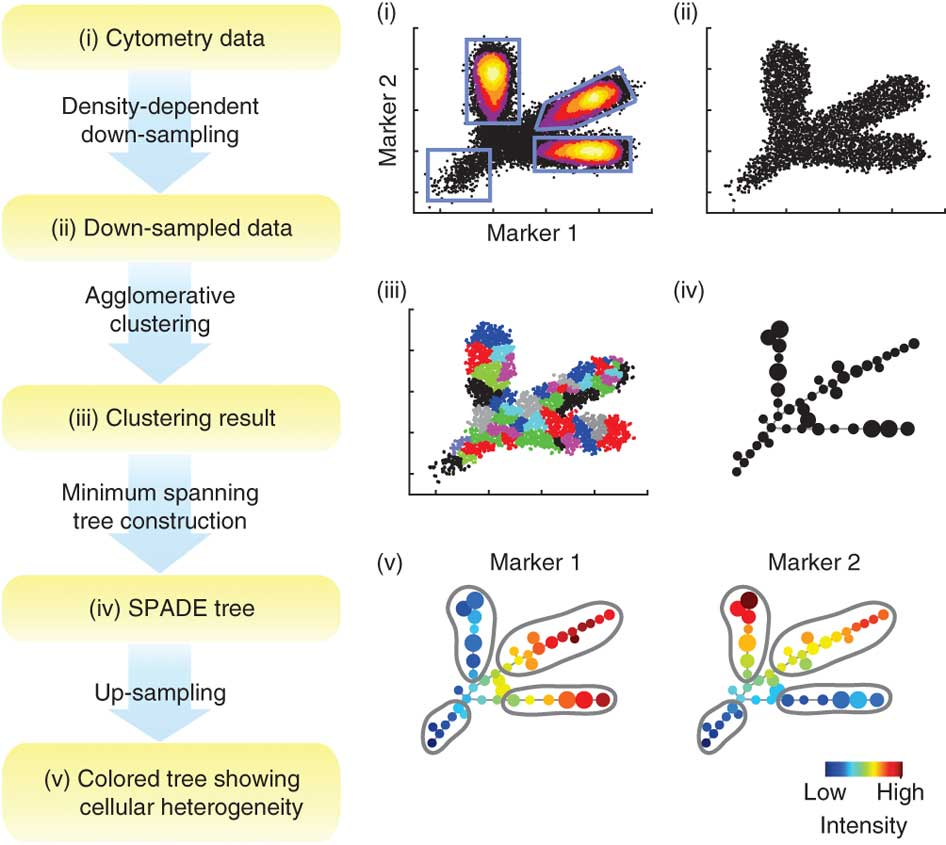
\includegraphics[width=0.45\textwidth]{Figures/SPADE-flowchart.jpg}
\end{center}
\caption{Overview of steps involved in the SPADE algorithm: Density-dependent downsampling, clustering, cluster preserving up-sampling, Minimum Spanning Tree construction, 2-D visualization.  Figure from \cite{}. }
\label{fig:spade_overview}
\end{figure}

%\subsection{Evaluating the effectiveness of SPADE}

While SPADE is a significant improvement over previous manual data analysis techniques, 
%several fundamental components of the underlying algorithm
we are concerned that its  sub-component algorithms and ad-hoc parameter settings may lead to inconsistent and potentially misleading outputs.  Because biologists interpret SPADE visualizations to support or refute hypotheses, it is important that SPADE and related cytometry analysis algorithms  yield reproducible results that do not  inject structure into visualizations that do not exist in the raw data. 

We examine the behavior of SPADE by generating synthetic datasets and comparing their known ground-truth structure to SPADE output visualizations.  Figure \ref{fig:spade_analysis} shows the results of this analysis for 3 synthetic datasets constructed by sampling points from  mixtures of Gaussian distributions in two dimensions.% centered at several cluster centers. 
 
We see that artificial structure is imposed when there is none

Shortening and thickening the branches complicates the underlying minimum spanning tree further, so we also tried running SPADE on this

Finally, as SPADE outputs a visualization highly dependent on there being an easily discoverable minimum spanning tree, we tested the algorithm on a dataset that is highly disconnected - four distinct, highly separated clusters.

\begin{figure}
\begin{center}
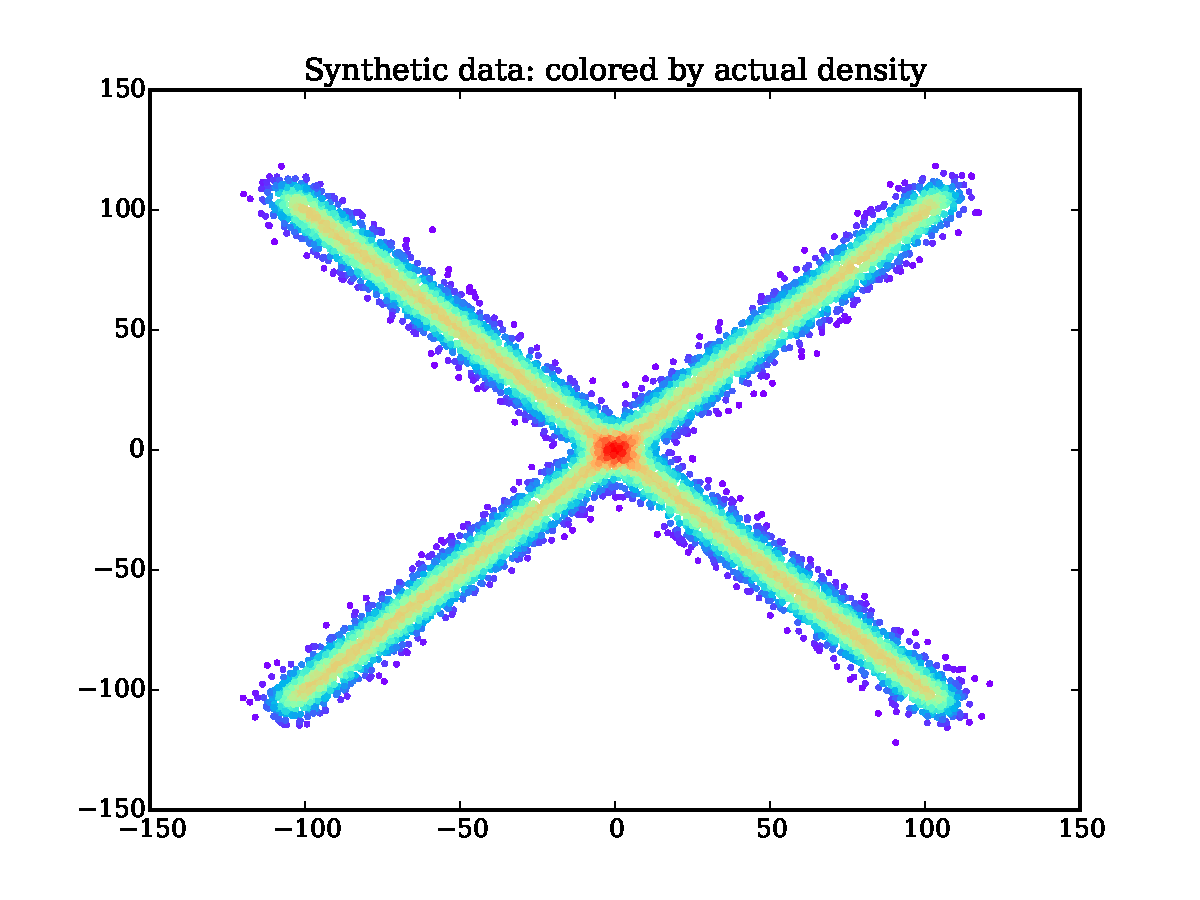
\includegraphics[width = 0.49\textwidth]{figures/synthetic_data.pdf}
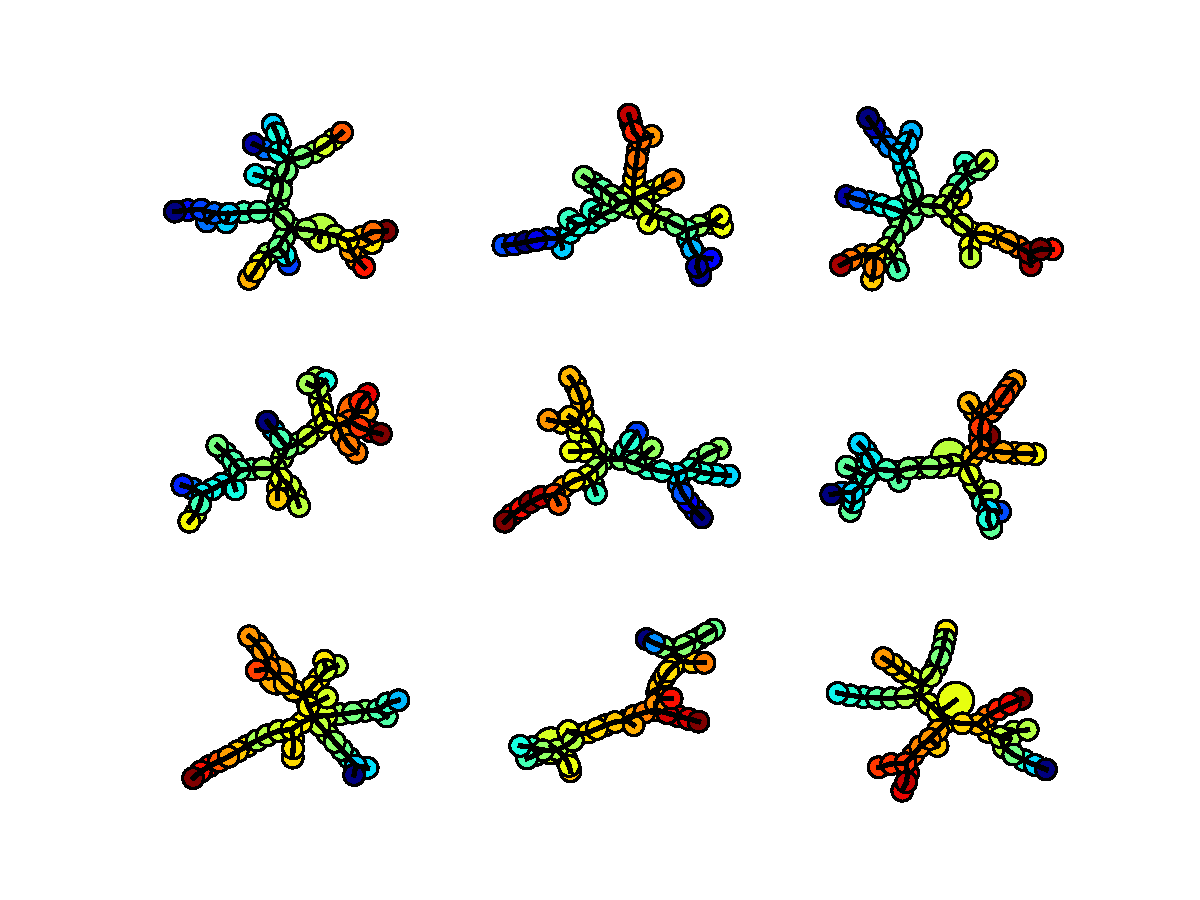
\includegraphics[width = 0.49\textwidth]{figures/spade_multiview.pdf}
\caption{CAPTION}
\label{fig:spade_analysis}
\end{center}
\end{figure}


%are poorly justified and ad-hoc.   For example, the method used to perform density dependent downsampling in the first step uses (without any motivating rationale) a radial measure (measured with $\ell_1$ distance) to estimate the density of points in a particular area. The potential shortcomings of this method are discussed further in Section 3. The choice of using force-directed-layout as a dimensionality reduction method are also not explored, and later (Section 4) we discuss alternate methods of embedding that allow good visualization. 

%In this section, we try and provide an evaluation of SPADE by generating synthetic data, which acts as a ground truth, and then comparing the output of SPADE to the shape of the synthetic data. We see that in many cases, SPADE creates artificial structure which distorts the true structure of the data. Furthermore, this artificial structure varies greatly due to the stochasticity of the density dependent downsampling step, making the algorithm quite inconsistent.

%\subsubsection{Experiments}

%Our experiments mainly involved generating synthetic data that was well separated, for example, by picking several distinct points on the plane, turning those into cluster centers, by sampling points from a Gaussian distribution, centered at the cluster centers. 

%Below is one such example of a dataset, with clusters colored to look more distinct, and cluster centers joined up with each other in the order they were produced.


We see that SPADE performs inconsistently and inaccurately on even simple synthetic datasets. While these datasets might not be identical to the single cell datasets on which SPADE is most commonly used, the popularity and diverse uses for the algorithm mean that it is especially important for it to be very robust, which is worryingly not the case.



\section{Density-Dependent Downsampling}
\label{sec:downsampling}
Both SPADE and FLOW-MAP algorithms for analyzing mass cytometry data involve density-dependent downsampling as a step in the data processing pipeline. This entails randomly omitting a subset of data points such that the probability of omitting a given point is positively correlated with the point’s local density in the full dataset.  Density-dependent downsampling is intended to serve two purposes:  First, it should increase the sensitivity to small clusters in successive clustering steps. Second, it should reduce computation cost of subsequent steps by reducing the overall number of points passed to the rest of the algorithm.

Density-dependent downsampling requires a way to estimate the local density at a point $p$, $D(p)$, to determine the probability of including $p$ in the sampled subset.  SPADE and FLOW-MAP estimate $D(p)$ by counting the number of points within a threshold L1-distance $r$ of $p$. However, this density estimation technique is inadequately justified.

To compare the accuracy of multiple density estimation algorithms, we performed numerical experiments with generated synthetic datasets. First, we drew 5000 points from a scikit-learn kernel density estimator \cite{} fit to 4 distinct cluster centers in 2 dimensions and 10 distinct cluster centers in 10 dimensions (Figure \ref{fig:ddd_data_2d}). The “ground truth” local density for each point was calculated by scoring the points using the fit kernel density estimator.  We then compared these ground truth densities to the output of four potential density estimation algorithms:

%\begin{figure}
%\begin{center}
%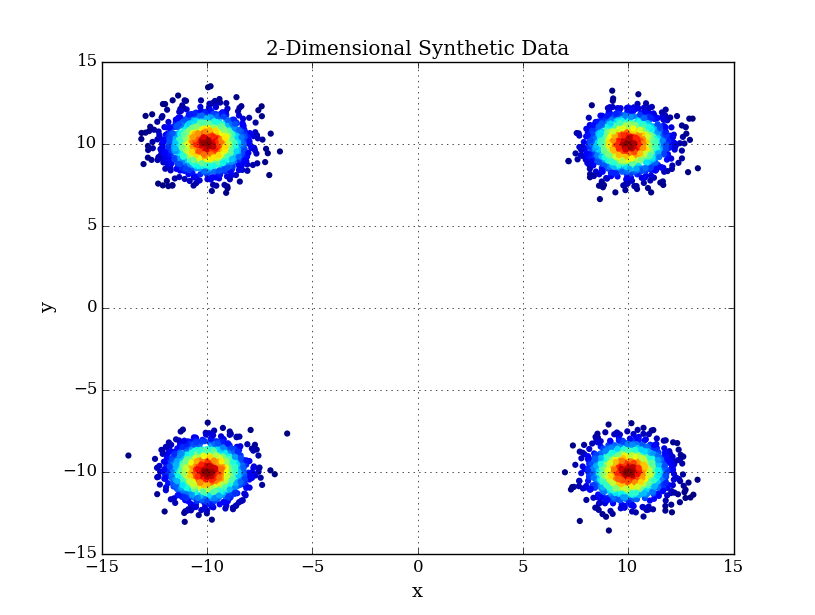
\includegraphics[width=0.35\textwidth]{Figures/ddd_data_2d.png}
%\end{center}
%\caption{Example 2-dimensional synthetic dataset generated for density estimation algorithm analysis.  Point color corresponds to ``ground truth" local density.}
%\label{fig:ddd_data_2d}
%\end{figure}

\begin{enumerate}
\item \textbf{Radius Threshold, L1:} The density estimation technique used by SPADE and FLOW-MAP. For each point $p$, the local density $D(p)$ is estimated as the count of points within a threshold L1-distance $r$ of $p$. 

\item \textbf{Radius Threshold, L2:} Identical to 1, except using $L2$ distance for the radius threshold $r$. 

\item \textbf{K-Nearest Neighbor, L1:} For each point $p$, find the $k$ points closest to $p$ by $L1$ distance.  The average normalized distance, $d$, between $p$ and each of these $k$ points in $m$ dimensions transformed as $\exp(d^m)$ (to improve linearity) is the estimated local density $D(p)$. 

\item \textbf{K-Nearest Neighbor, L2:} Identical to 3, except using $L2$ distance to find nearest neighbors.

%\item \textbf{scikit-learn Kernel Density Estimator:} scikit-learn’s built-in kernel density estimator using cross-validation to set the bandwidth.

\end{enumerate}

Figure \ref{fig:ddd_results} shows algorithm performance for a range of parameter values $r$ and $k$ measured as the $R^2$ coefficient of determination of a linear model fit to the predicted density versus the ground truth density.   Specific results of interest are the maximum $R^2$ value for each algorithm (indicating the approximate maximum accuracy of the algorithm on this particular dataset), the range of parameter values corresponding to high $R^2$ coefficients, and the general trend of the $R^2$ values over the parameter space. 

Although the Radius Threshold density estimator has a higher maximum $R^2$ value than the K-Nearest Neighbor estimator in both 2 and 10 dimensions, the K-Nearest Neighbor estimator provides much more stable estimates over a range of $k$ and accuracy monotonically increasing with $k$. These stability and monotonicity properties would make the K-Nearest Neighbor estimator a better choice for algorithms such as SPADE and FLOW-MAP.  This is especially true considering the difficulty of choosing an appropriate value of $r$ or $k$ given an experimental dataset.  Unlike the synthesized datasets used for algorithm analysis, cytometry datasets input to SPADE and FLOW-MAP do not come with a ``ground truth'' density.  SPADE arbitrarily chooses $r$ to be a user-selected parameter $\alpha$ times the median 1-nearest neighbor distance between a randomly selected subset of 2000 data points. Using this heuristic on our synthesized datasets corresponds to the red dotted line in Figure \ref{fig:ddd_results} and results in a suboptimal density estimation. The K-Nearest Neighbor estimator avoids this ``needle in a haystack’’ parameter selection problem.

Figure \ref{fig:ddd_results} also indicates that using $L1$ distance results in a wider range of high-accuracy values of $r$ for the Radius Threshold estimation algorithm, but that the choice of distance metric does not have a major effect on density estimation accuracy for the K-Nearest Neighbor algorithm.  This further supports the stability of the K-Nearest Neighbor algorithm.  

\begin{figure*}
\begin{center}
\subfigure[50-Dimensions]{
	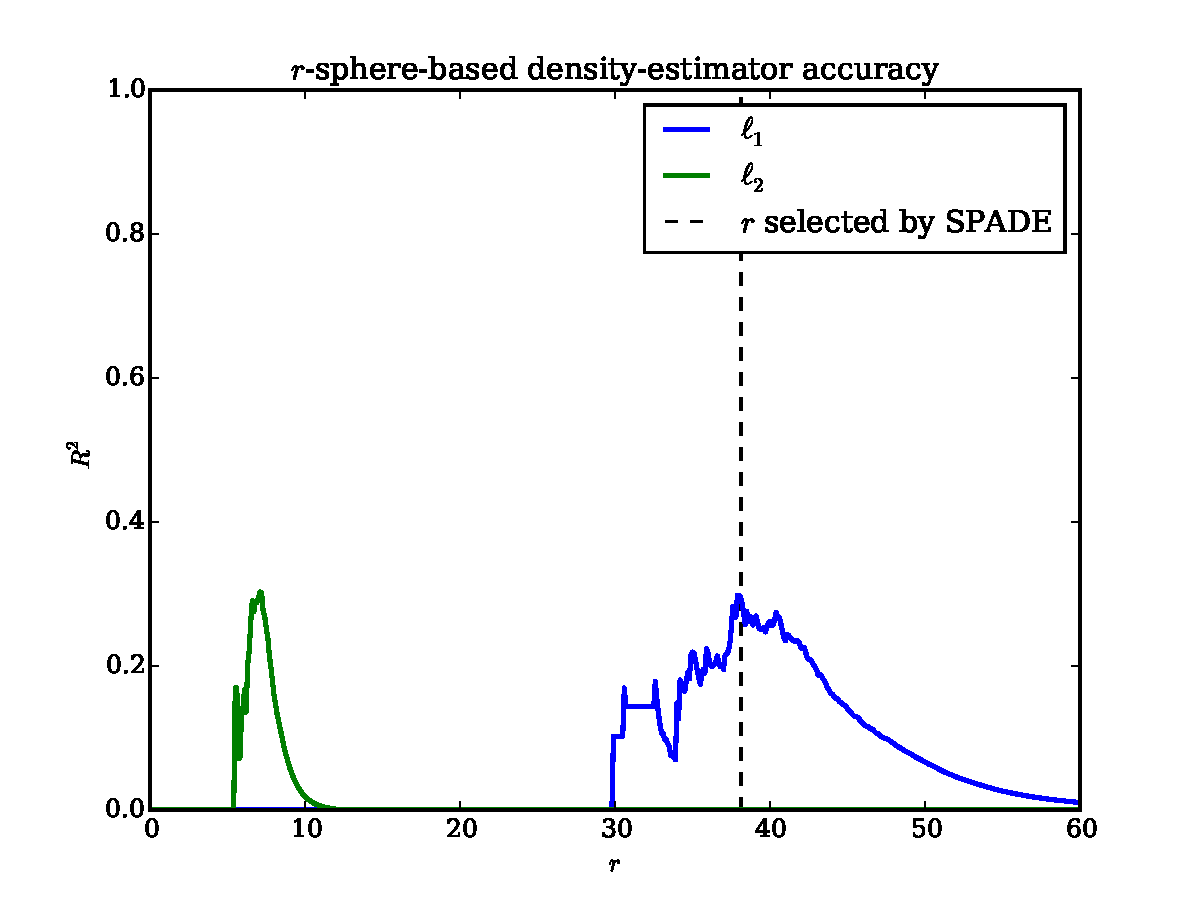
\includegraphics[width = 0.49\textwidth]{figures/r-sphere-50D-blobs.pdf}
   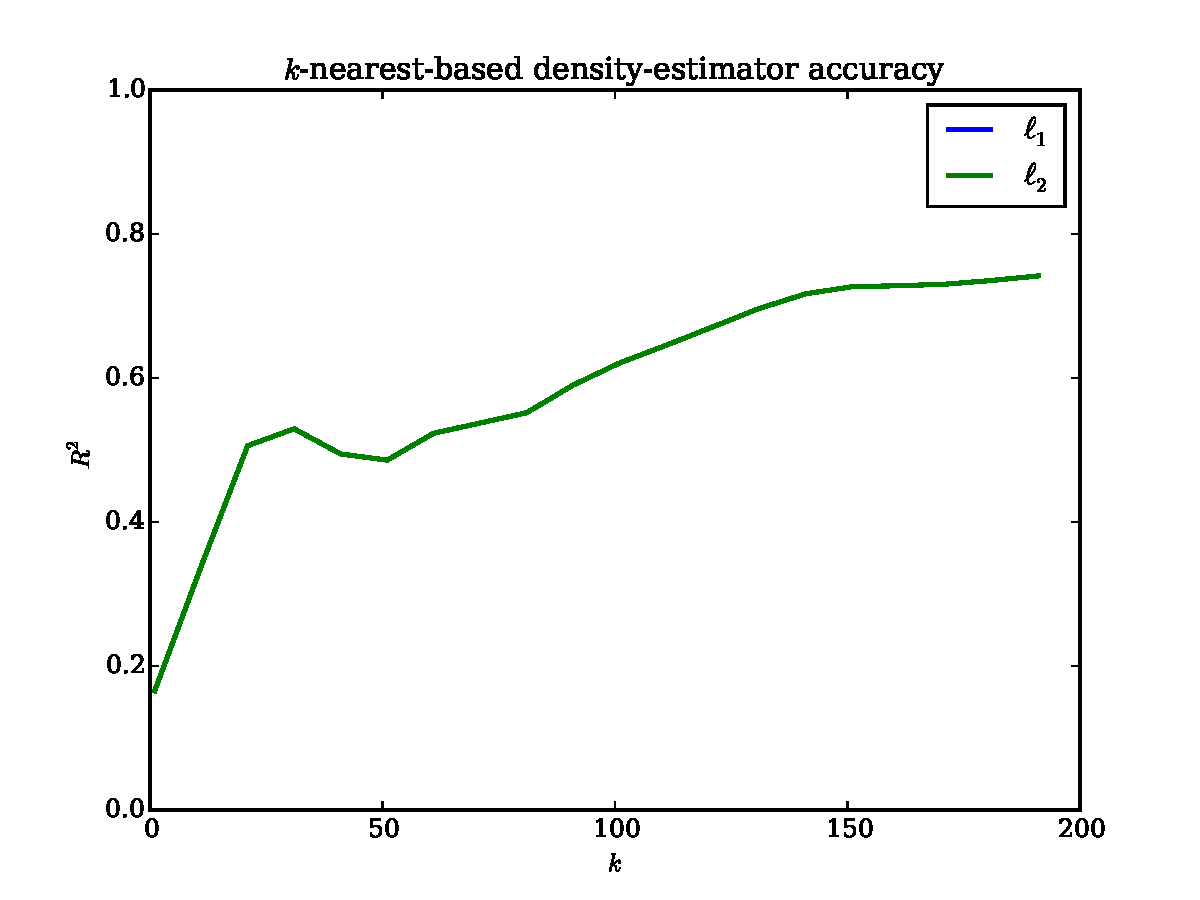
\includegraphics[width = 0.49\textwidth]{figures/k-nearest-50D-blobs.pdf}
   \label{fig:ddd_results_50d}
 }

\subfigure[10-Dimensions]{
	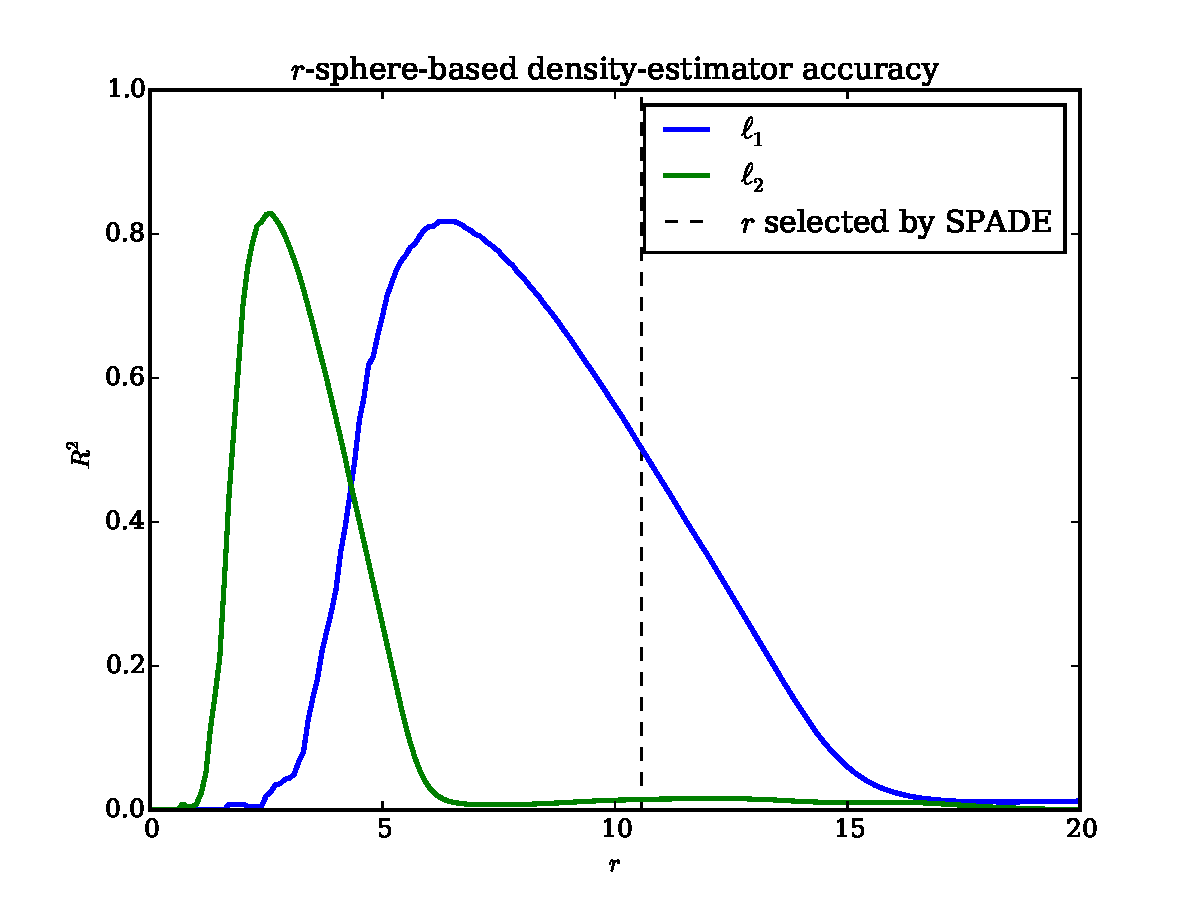
\includegraphics[width = 0.49\textwidth]{figures/r-sphere-10D-blobs.pdf}
   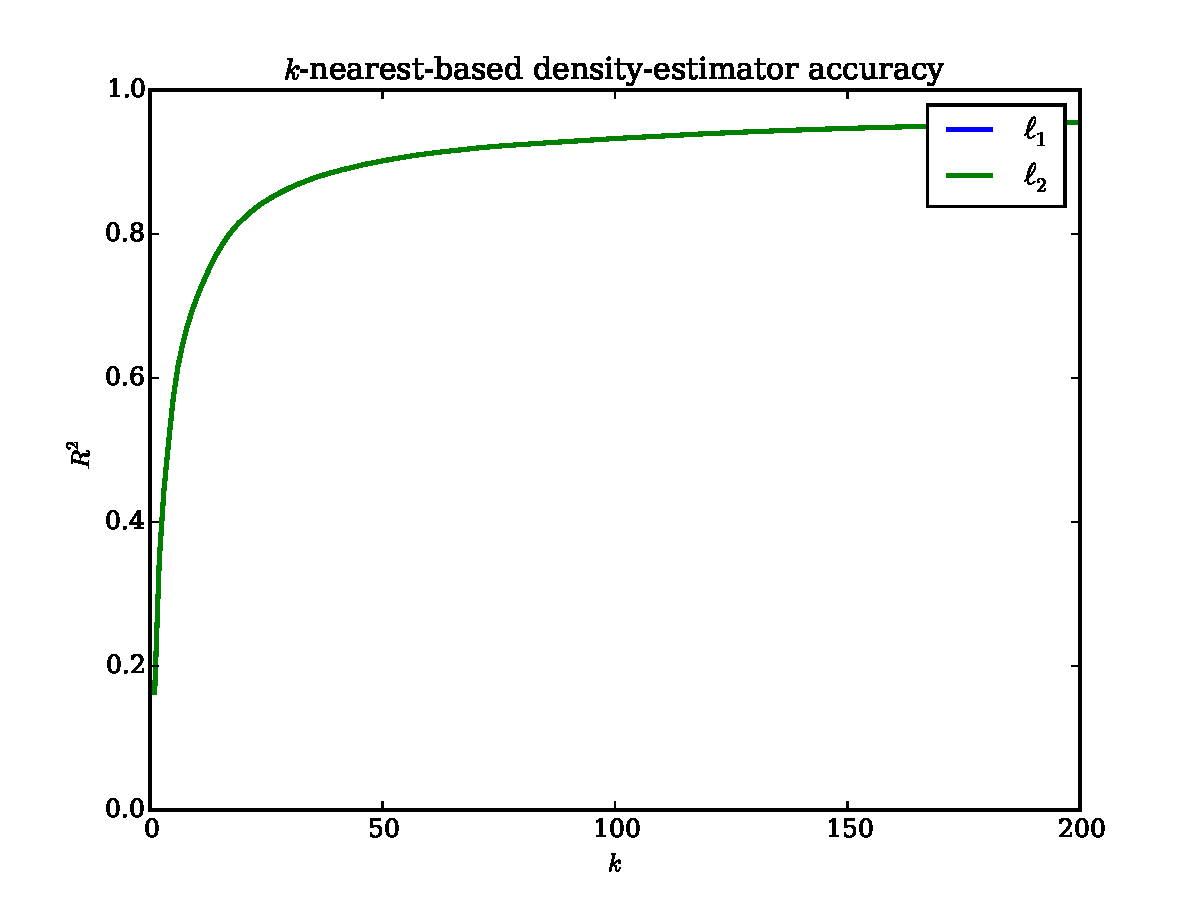
\includegraphics[width = 0.49\textwidth]{figures/k-nearest-10D-blobs.pdf}
   \label{fig:ddd_results_50d}
 }

\caption{CAPTION}
\label{fig:ddd_results}
\end{center}
\end{figure*}

FINAL TAKEAWAY?

\begin{figure}
\begin{center}

\subfigure[Synthetic Dataset]{
	\centering
	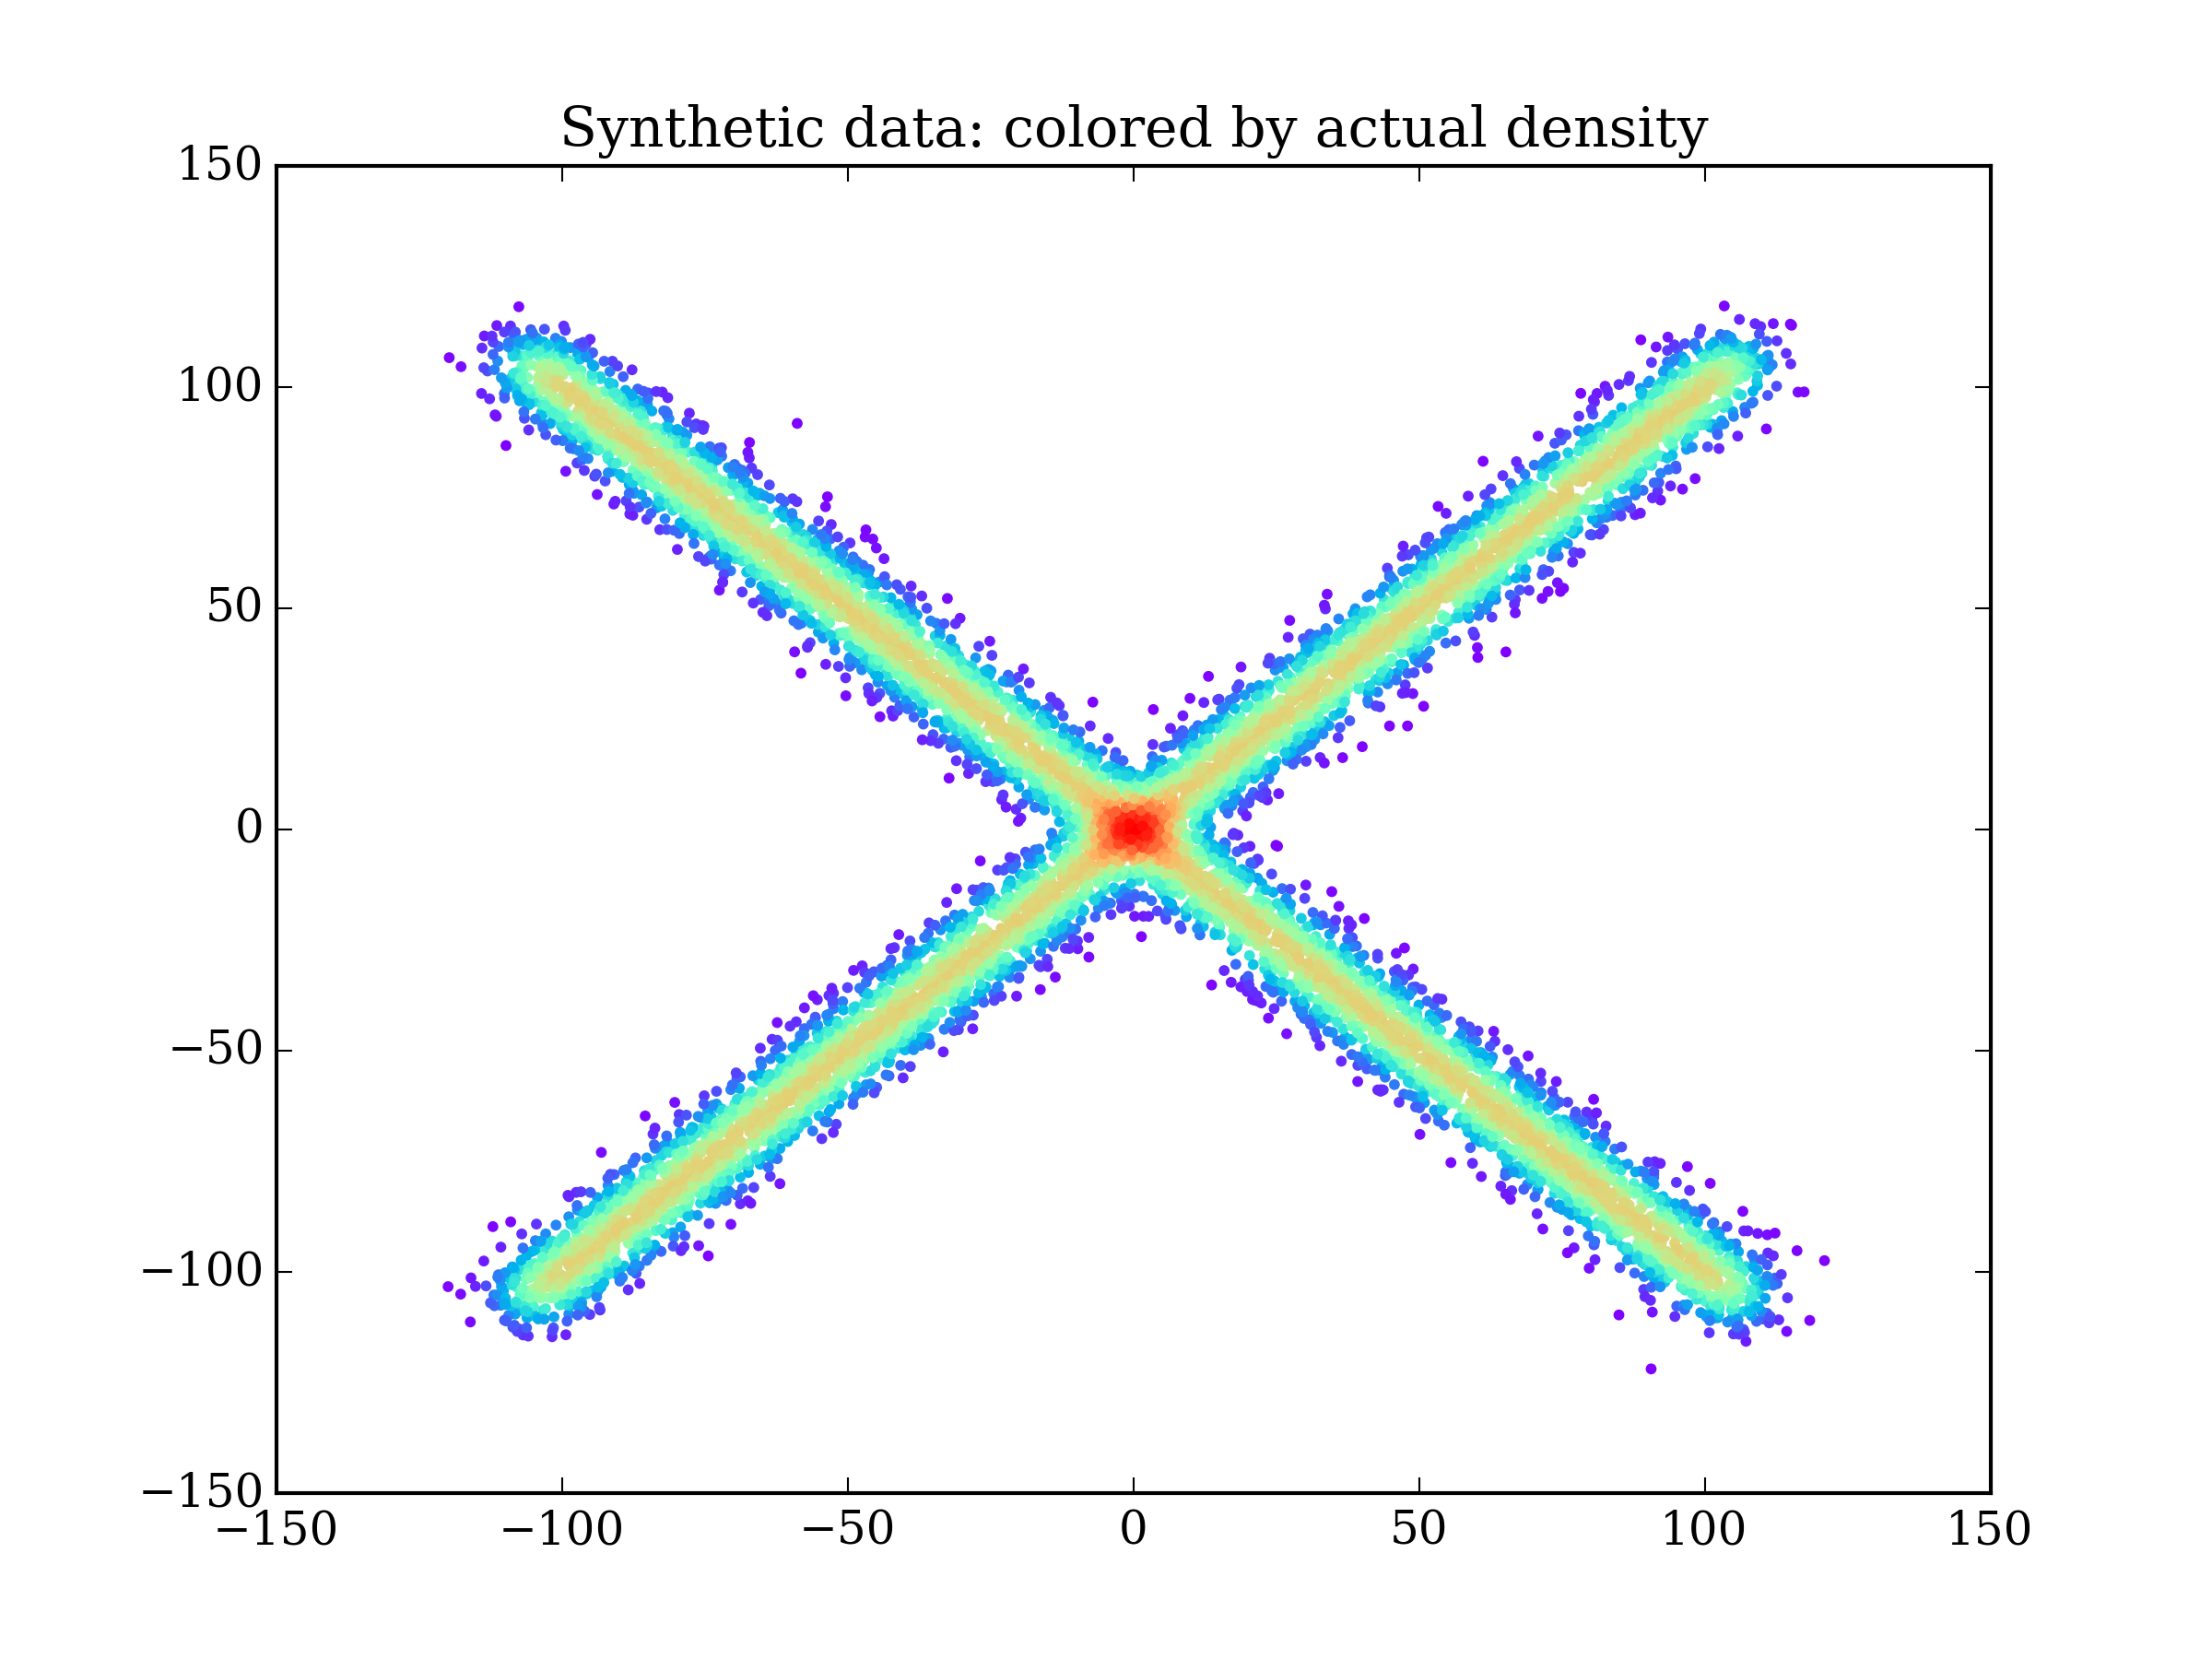
\includegraphics[width = 0.40\textwidth]{figures/synthetic_data.png}
   \label{fig:ddd_effects_syn}
 }

\subfigure[Downsampled with Radius Threshold density estimation]{
	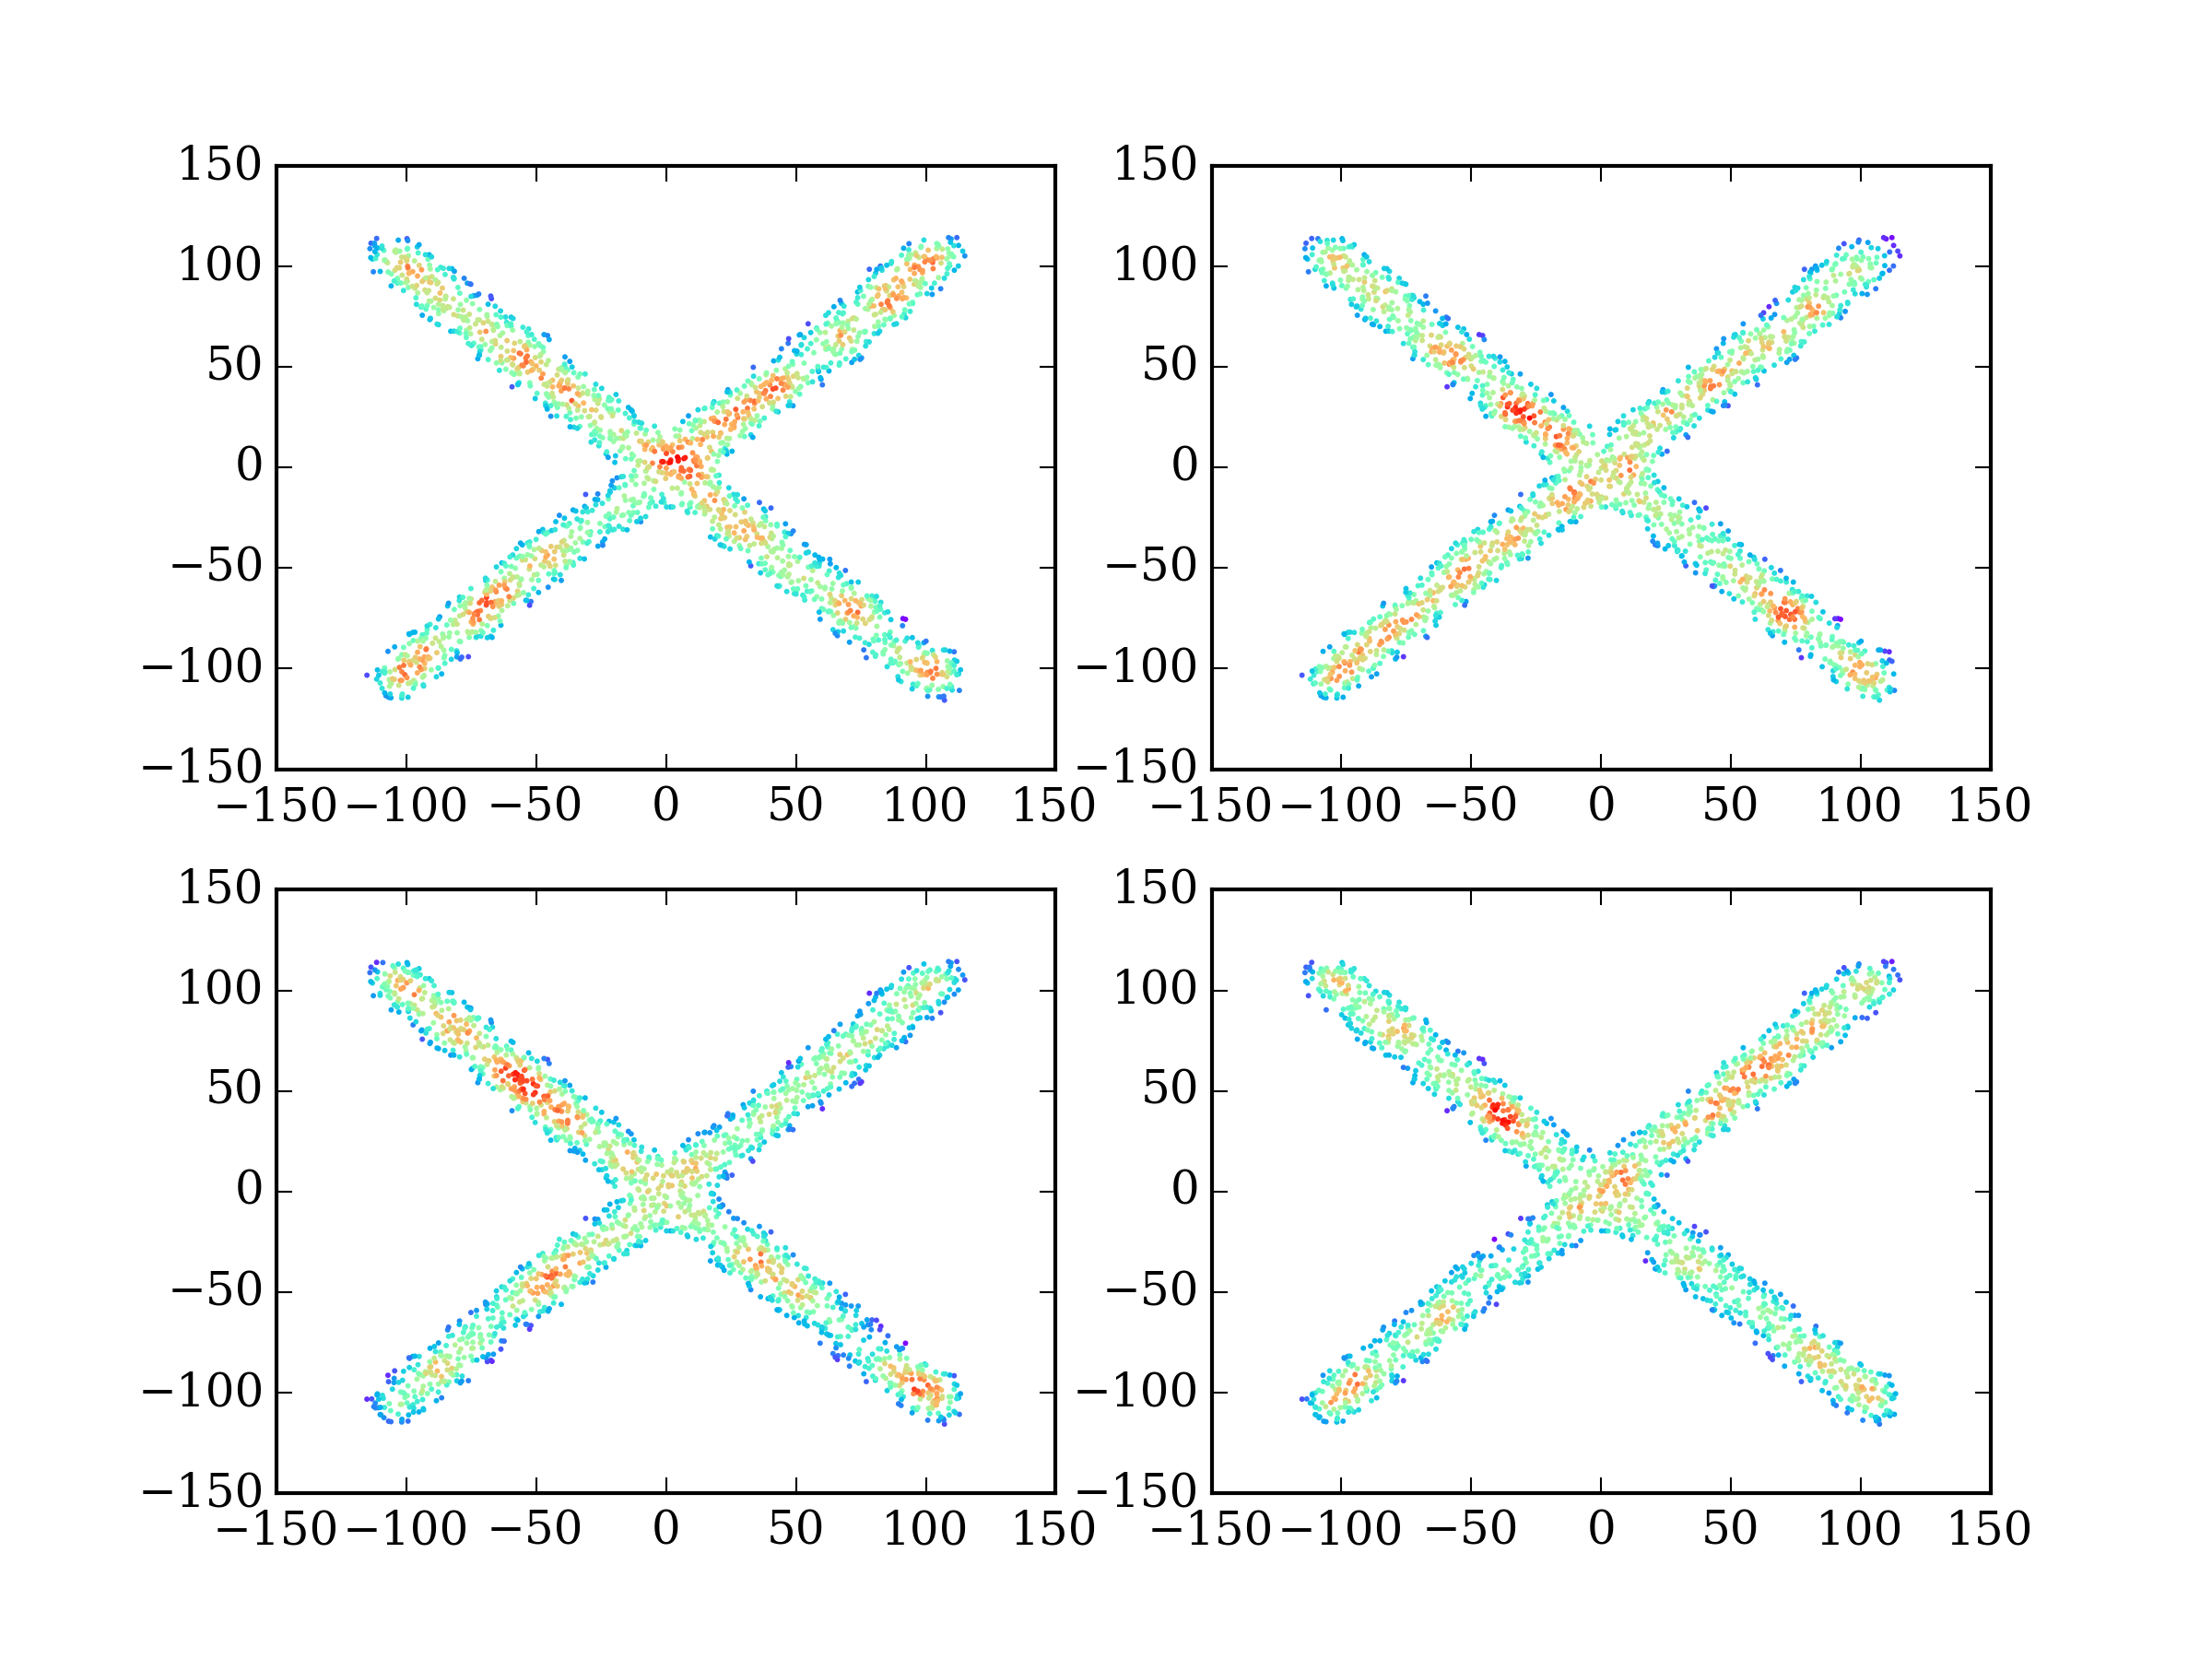
\includegraphics[width = 0.50\textwidth]{figures/synthetic_data_downsampled_r.png}
   \label{fig:ddd_effects_r}
 }

\subfigure[Downsampled with K-Nearest Neighbor density estimation]{
	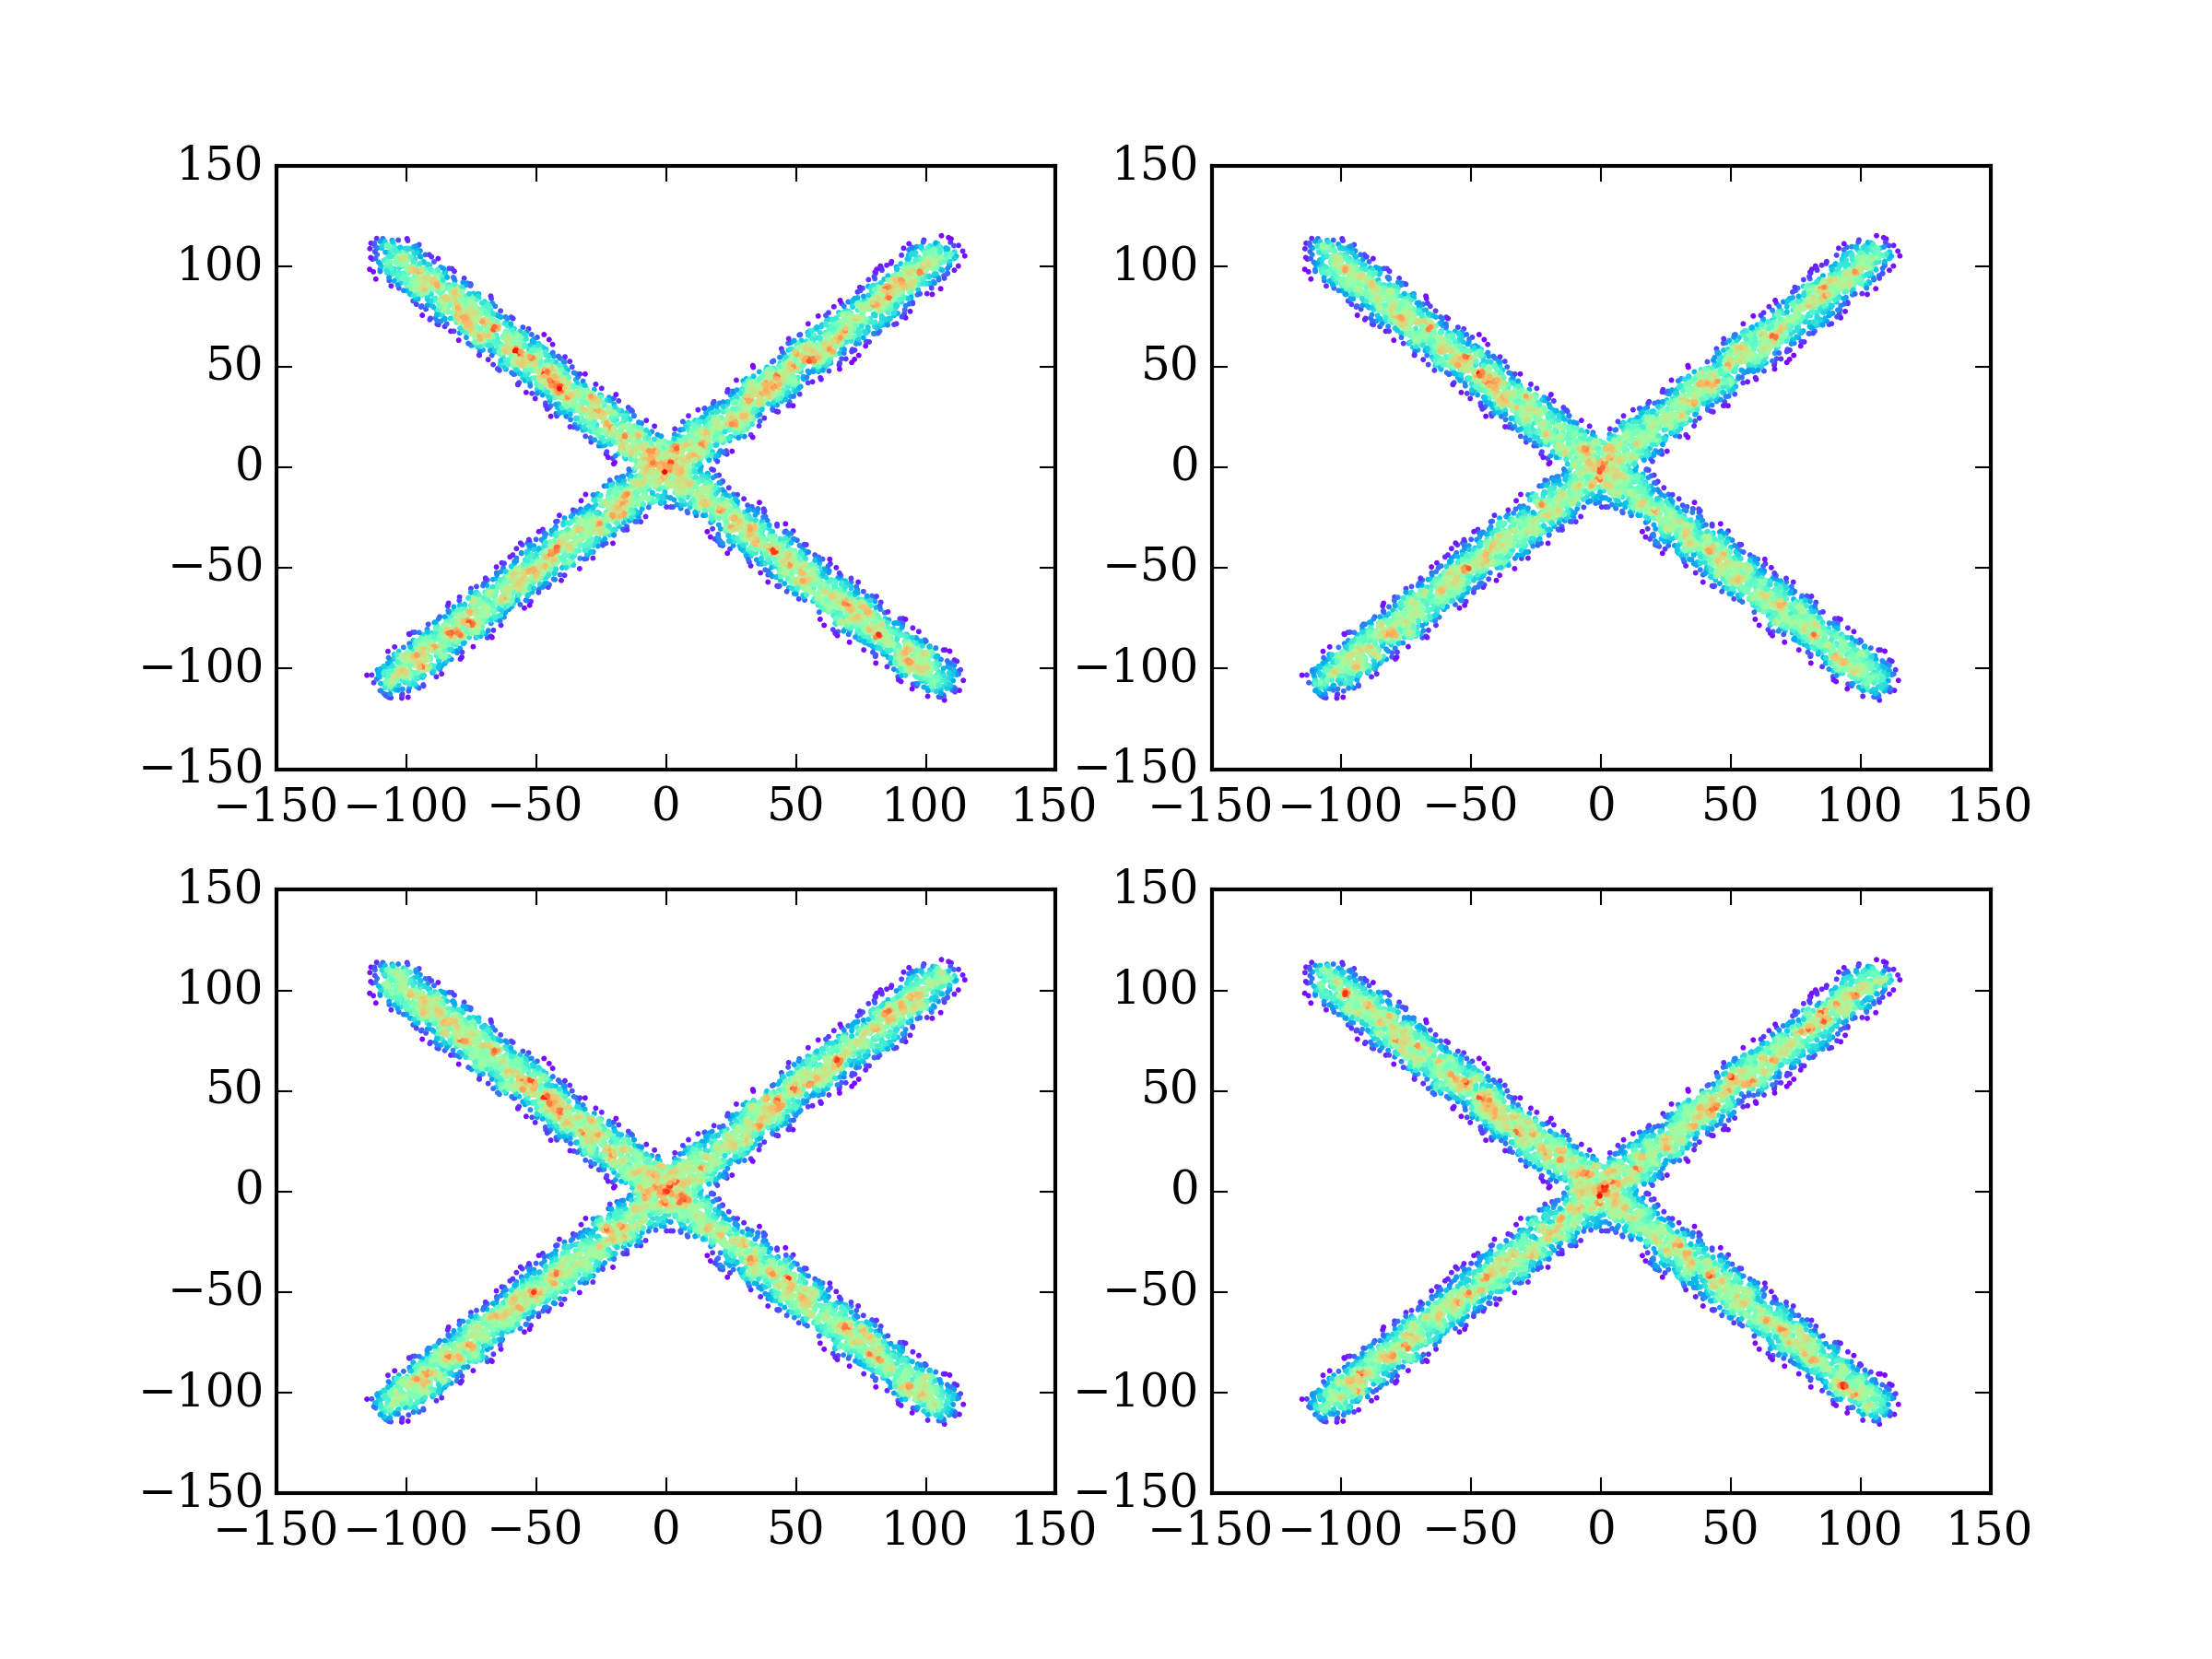
\includegraphics[width = 0.50\textwidth]{figures/synthetic_data_downsampled_k.png}
   \label{fig:ddd_effects_k}
 }

\caption{CAPTION}
\label{fig:ddd_effects}
\end{center}
\end{figure}


\section{Approximate Tree-Preserving Embedding}
Background / motivation
A primary motivation for creating a 2D embedding is to reveal cluster structure in an intuitive, human-readable representation. Ideally, such an embedding simultaneously preserves clusters and the relations between clusters---similar items within a cluster should be near each other, similar clusters should be close together in the embedding, etc. There are many ways to produce such an embedding, including linear methods like principal component analysis (PCA), and nonlinear methods like Isomap \cite{}, Locally Linear Embedding \cite{}, and t-SNE \cite{}. PCA can be shown to minimize the sum of squared reconstruction errors, which induces an embedding that preserves the largest pairwise distances with high fidelity, and places less emphasis on preserving the smallest pairwise distances. In cases where the clusters are linearly separable in the target dimensionality, the embedding produced by PCA is a suitable visualization. Because clusters are often not linearly separable in real data, nonlinear methods have been developed. Techniques like Isomap and Locally Linear Embedding construct neighborhood graphs and preserve distances (e.g. shortest-path distances) within these graphs, so they can sometimes outperform PCA at local neighborhood preservation and other metrics. However, they may distort or introduce structure not present in the original data, and are sensitive to user-defined settings of free parameters.

Recent work \cite{tpe} constructively produces a low-dimensional embedding such that the results of hierarchical clustering are identical in the original data and the embedding. The “Tree-Preserving Embedding” algorithm achieves strong theoretical guarantees, but its cost is cubic in the size of the input dataset $n$ (with large leading constants), is prohibitively slow when $n > 300$, and is somewhat complicated to implement correctly.

Here we attempt to develop a simpler low-dimensional embedding technique that also approximately preserves both fine- and coarse-grained cluster structure.

Algorithm
We propose “Approximate TPE,” a simpler approximation that is also naively $O(n^3)$, but provides a more direct route to further performance optimization. Approximate TPE (1) computes an agglomerative hierarchical cluster tree, (2) extracts a pairwise distance matrix $A$ from this tree, and (3) approximately preserves these distances in a low-dimensional embedding. The user can select any linkage to construct the cluster tree (we show results for single-, median-, average, ward-, and complete- linkage). The entries $A_{ij}$ of the pairwise distance matrix are cophenetic distances: the height in the cluster tree at which points $i$ and $j$ are merged. A low-dimensional embedding that approximately preserves these distances is then computed by multidimensional scaling (MDS) \cite{}.


Comparison on benchmark data
We tested the method on (1) two Gaussians, (2) Gaussians on hypercubes, (3) handwritten digit data ($n=1797$), (4) ???.

This approximation outperforms competing algorithms when measured by neighborhood preservation.

Competing algorithms: PCA, KPCA (RBF kernel), t-SNE, Isomap, LLE. All with target-dimensionality of 2.

However, depending on the choice of linkage, sometimes the algorithm collapses many similar points into small, dense regions of the embedding, which is visually unreadable. [propose solutions? e.g. we might be able to solve this by rescaling the entries of the cophenetic distance matrix? … tried a couple different things: one thing that works is to scale by the Euclidean distance… see comment… ]
Two functional approaches to tackling this problem: (1) rescale smallest distances in input matrix (for example, replace smallest distances with raw Euclidean distances), (2) after MDS embedding has been computed, tweak the locations such that very small distances are “high-stress”: i.e. push apart any pair of points that’s too close together

[to-do: measure of tree-preserving-ness]

[to-do: procrustes analysis on synthetic data]

[to-do: measure cluster-preservation somehow? Estimate number of clusters in original data and and low-dimensional embedding and compare?]

[to-do: apply to biological data]

Future work
Future work will address the computational cost of the algorithm and the “crowding problem,” as well as providing better heuristics for choosing the linkage type.

Construction of the hierarchical cluster tree is naively an $O(n^3)$ operation, but that can be reduced to nearly linear-time by “bootstrapping” with a tree that is much cheaper to construct (such as a KD-tree) \cite{fast_agglom_clust_kdtree}. Another approach to accelerate construction of the cluster tree is to use a sparse $k$-nearest-neighbors graph \cite{fast_agglom_clust_knn}.

Computing a low-dimensional embedding from the distance matrix via MDS is also naively $O(n^3)$, but there has been some research into fast approximations for MDS.
$O(n \log n)$ divide-and-conquer approach: http://www.cs.ucla.edu/~weiwang/paper/CIMCV06.pdf
Nystrom approaches: FastMap, MetricMap, Landmark MDS

[expand this section?]


\section{FLOW-MAP}
Recent work proposed ‘FLOW-MAP’ as an algorithm for 2D visualization of the results of mass cytometry data with a time component. In these experiments, a population of cells is sampled at several time intervals, yielding a series of snapshots of the population over time. The paper introducing FLOW-MAP examined three techniques for stem cell reprogramming. The combined 2D map should illustrate whether the three techniques vary in their end-points / the intermediate cellular states visited by the population over the course of the procedures. In other words, we would like to learn a “progression axis” for each reprogramming technique that describes the progression of the cellular population over time, and we would like to produce an accurate 2D representation of the data.
The authors of the algorithm recognize that the combination of stochastic down-sampling and imposition of very sparse constraints on the final visualization can lead to inconsistency in the results of SPADE. To address these limitations, they proceed by constructing a denser constraint graph, where nodes are clusters and edges are distances between cluster centers. Sparsity is induced by a series of rules for whether an edge should be included in the graph. Edges are further filtered by adjacency in time: two datapoints can only share an edge in this graph if they were observed in either the same time step or in consecutive timesteps. The visualization coordinates are then computed by applying force-directed layout to this slightly denser graph.
However, this approach raises some fresh concerns. For example, imposing the constraint of timestep adjacency may obscure the presence of populations that are present at multiple time points that are not adjacent, since they cannot be connected directly by edges. Other constraints imposed by user-defined parameters make it likely for many points to be connected in “chains,” where each point’s degree is 2: when combined with force-directed layout, this makes the embedding seem to contain well separated clusters with intermediates stretched along a thin line between them. It is unclear if this is an accurate depiction of the data.
To test whether these methods are distorting the data, we need to compare the results obtained using these methods to the results obtained from using simpler methods that are easier to reason about. To this end we cast the problem as a supervised problem: from a cellular “feature vector” predict what time it was measured. If we can perform this task well, then we have probably learned a good progression function.


\bibliography{example_paper}
\bibliographystyle{icml2015}

\end{document} 


% This document was modified from the file originally made available by
% Pat Langley and Andrea Danyluk for ICML-2K. This version was
% created by Lise Getoor and Tobias Scheffer, it was slightly modified  
% from the 2010 version by Thorsten Joachims & Johannes Fuernkranz, 
% slightly modified from the 2009 version by Kiri Wagstaff and 
% Sam Roweis's 2008 version, which is slightly modified from 
% Prasad Tadepalli's 2007 version which is a lightly 
% changed version of the previous year's version by Andrew Moore, 
% which was in turn edited from those of Kristian Kersting and 
% Codrina Lauth. Alex Smola contributed to the algorithmic style files.  
